% Options for packages loaded elsewhere
\PassOptionsToPackage{unicode}{hyperref}
\PassOptionsToPackage{hyphens}{url}
%
\documentclass[
  man]{apa6}
\usepackage{amsmath,amssymb}
\usepackage{lmodern}
\usepackage{iftex}
\ifPDFTeX
  \usepackage[T1]{fontenc}
  \usepackage[utf8]{inputenc}
  \usepackage{textcomp} % provide euro and other symbols
\else % if luatex or xetex
  \usepackage{unicode-math}
  \defaultfontfeatures{Scale=MatchLowercase}
  \defaultfontfeatures[\rmfamily]{Ligatures=TeX,Scale=1}
\fi
% Use upquote if available, for straight quotes in verbatim environments
\IfFileExists{upquote.sty}{\usepackage{upquote}}{}
\IfFileExists{microtype.sty}{% use microtype if available
  \usepackage[]{microtype}
  \UseMicrotypeSet[protrusion]{basicmath} % disable protrusion for tt fonts
}{}
\makeatletter
\@ifundefined{KOMAClassName}{% if non-KOMA class
  \IfFileExists{parskip.sty}{%
    \usepackage{parskip}
  }{% else
    \setlength{\parindent}{0pt}
    \setlength{\parskip}{6pt plus 2pt minus 1pt}}
}{% if KOMA class
  \KOMAoptions{parskip=half}}
\makeatother
\usepackage{xcolor}
\usepackage{graphicx}
\makeatletter
\def\maxwidth{\ifdim\Gin@nat@width>\linewidth\linewidth\else\Gin@nat@width\fi}
\def\maxheight{\ifdim\Gin@nat@height>\textheight\textheight\else\Gin@nat@height\fi}
\makeatother
% Scale images if necessary, so that they will not overflow the page
% margins by default, and it is still possible to overwrite the defaults
% using explicit options in \includegraphics[width, height, ...]{}
\setkeys{Gin}{width=\maxwidth,height=\maxheight,keepaspectratio}
% Set default figure placement to htbp
\makeatletter
\def\fps@figure{htbp}
\makeatother
\setlength{\emergencystretch}{3em} % prevent overfull lines
\providecommand{\tightlist}{%
  \setlength{\itemsep}{0pt}\setlength{\parskip}{0pt}}
\setcounter{secnumdepth}{-\maxdimen} % remove section numbering
% Make \paragraph and \subparagraph free-standing
\ifx\paragraph\undefined\else
  \let\oldparagraph\paragraph
  \renewcommand{\paragraph}[1]{\oldparagraph{#1}\mbox{}}
\fi
\ifx\subparagraph\undefined\else
  \let\oldsubparagraph\subparagraph
  \renewcommand{\subparagraph}[1]{\oldsubparagraph{#1}\mbox{}}
\fi
\newlength{\cslhangindent}
\setlength{\cslhangindent}{1.5em}
\newlength{\csllabelwidth}
\setlength{\csllabelwidth}{3em}
\newlength{\cslentryspacingunit} % times entry-spacing
\setlength{\cslentryspacingunit}{\parskip}
\newenvironment{CSLReferences}[2] % #1 hanging-ident, #2 entry spacing
 {% don't indent paragraphs
  \setlength{\parindent}{0pt}
  % turn on hanging indent if param 1 is 1
  \ifodd #1
  \let\oldpar\par
  \def\par{\hangindent=\cslhangindent\oldpar}
  \fi
  % set entry spacing
  \setlength{\parskip}{#2\cslentryspacingunit}
 }%
 {}
\usepackage{calc}
\newcommand{\CSLBlock}[1]{#1\hfill\break}
\newcommand{\CSLLeftMargin}[1]{\parbox[t]{\csllabelwidth}{#1}}
\newcommand{\CSLRightInline}[1]{\parbox[t]{\linewidth - \csllabelwidth}{#1}\break}
\newcommand{\CSLIndent}[1]{\hspace{\cslhangindent}#1}
\ifLuaTeX
\usepackage[bidi=basic]{babel}
\else
\usepackage[bidi=default]{babel}
\fi
\babelprovide[main,import]{american}
% get rid of language-specific shorthands (see #6817):
\let\LanguageShortHands\languageshorthands
\def\languageshorthands#1{}
% Manuscript styling
\usepackage{upgreek}
\captionsetup{font=singlespacing,justification=justified}

% Table formatting
\usepackage{longtable}
\usepackage{lscape}
% \usepackage[counterclockwise]{rotating}   % Landscape page setup for large tables
\usepackage{multirow}		% Table styling
\usepackage{tabularx}		% Control Column width
\usepackage[flushleft]{threeparttable}	% Allows for three part tables with a specified notes section
\usepackage{threeparttablex}            % Lets threeparttable work with longtable

% Create new environments so endfloat can handle them
% \newenvironment{ltable}
%   {\begin{landscape}\centering\begin{threeparttable}}
%   {\end{threeparttable}\end{landscape}}
\newenvironment{lltable}{\begin{landscape}\centering\begin{ThreePartTable}}{\end{ThreePartTable}\end{landscape}}

% Enables adjusting longtable caption width to table width
% Solution found at http://golatex.de/longtable-mit-caption-so-breit-wie-die-tabelle-t15767.html
\makeatletter
\newcommand\LastLTentrywidth{1em}
\newlength\longtablewidth
\setlength{\longtablewidth}{1in}
\newcommand{\getlongtablewidth}{\begingroup \ifcsname LT@\roman{LT@tables}\endcsname \global\longtablewidth=0pt \renewcommand{\LT@entry}[2]{\global\advance\longtablewidth by ##2\relax\gdef\LastLTentrywidth{##2}}\@nameuse{LT@\roman{LT@tables}} \fi \endgroup}

% \setlength{\parindent}{0.5in}
% \setlength{\parskip}{0pt plus 0pt minus 0pt}

% Overwrite redefinition of paragraph and subparagraph by the default LaTeX template
% See https://github.com/crsh/papaja/issues/292
\makeatletter
\renewcommand{\paragraph}{\@startsection{paragraph}{4}{\parindent}%
  {0\baselineskip \@plus 0.2ex \@minus 0.2ex}%
  {-1em}%
  {\normalfont\normalsize\bfseries\itshape\typesectitle}}

\renewcommand{\subparagraph}[1]{\@startsection{subparagraph}{5}{1em}%
  {0\baselineskip \@plus 0.2ex \@minus 0.2ex}%
  {-\z@\relax}%
  {\normalfont\normalsize\itshape\hspace{\parindent}{#1}\textit{\addperi}}{\relax}}
\makeatother

% \usepackage{etoolbox}
\makeatletter
\patchcmd{\HyOrg@maketitle}
  {\section{\normalfont\normalsize\abstractname}}
  {\section*{\normalfont\normalsize\abstractname}}
  {}{\typeout{Failed to patch abstract.}}
\patchcmd{\HyOrg@maketitle}
  {\section{\protect\normalfont{\@title}}}
  {\section*{\protect\normalfont{\@title}}}
  {}{\typeout{Failed to patch title.}}
\makeatother

\usepackage{xpatch}
\makeatletter
\xapptocmd\appendix
  {\xapptocmd\section
    {\addcontentsline{toc}{section}{\appendixname\ifoneappendix\else~\theappendix\fi\\: #1}}
    {}{\InnerPatchFailed}%
  }
{}{\PatchFailed}
\keywords{mental simulation, object orientation, mental rotation, language comprehension\newline\indent Word count: 5,138 words in total; Introduction: 1,242 words}
\DeclareDelayedFloatFlavor{ThreePartTable}{table}
\DeclareDelayedFloatFlavor{lltable}{table}
\DeclareDelayedFloatFlavor*{longtable}{table}
\makeatletter
\renewcommand{\efloat@iwrite}[1]{\immediate\expandafter\protected@write\csname efloat@post#1\endcsname{}}
\makeatother
\usepackage{csquotes}
\usepackage{caption}
\usepackage{float}
\ifLuaTeX
  \usepackage{selnolig}  % disable illegal ligatures
\fi
\IfFileExists{bookmark.sty}{\usepackage{bookmark}}{\usepackage{hyperref}}
\IfFileExists{xurl.sty}{\usepackage{xurl}}{} % add URL line breaks if available
\urlstyle{same} % disable monospaced font for URLs
\hypersetup{
  pdftitle={Investigating Object Orientation Effects Across 18 Languages},
  pdfauthor={Sau-Chin Chen1, Erin Buchanan2, Zoltan Kekecs3,4, Jeremy K. Miller5, Anna Szabelska6, Balazs Aczel3, Pablo Bernabeu7, Patrick Forscher8,9, Attila Szuts3, Zahir Vally10, Ali H. Al-Hoorie11, Mai Helmy12,13, Caio Santos Alves da Silva14, Luana Oliveira da Silva14, Yago Luksevicius de Moraes14, Rafael Ming C. S. Hsu14, Anthonieta Looman Mafra14, Jaroslava V. Valentova14, Marco Antonio Correa Varella14, Barnaby Dixon15, Kim Peters15, Nik Steffens15, Omid Ghaesmi16, Andrew Roberts16, Robert M. Ross16, Ian D. Stephen16,17, Marina Milyavskaya18, Kelly Wang18, Kaitlyn M. Werner18, Dawn L. Holford19, Miroslav Sirota19, Thomas Rhys Evans20, Dermot Lynott7, Bethany M. Lane21, Danny Riis21, Glenn P. Williams22, Chrystalle B. Y. Tan23, Alicia Foo24, Steve M. J. Janssen24, Nwadiogo Chisom Arinze25, Izuchukwu Lawrence Gabriel Ndukaihe25, David Moreau26, Brianna Jurosic27, Brynna Leach27, Savannah Lewis27, Peter R. Mallik27, Kathleen Schmidt28, William J. Chopik29, Leigh Ann Vaughn30, Manyu Li31, Carmel A. Levitan32, Daniel Storage33, Carlota Batres34, Janina Enachescu35, Jerome Olsen35, Martin Voracek35, Claus Lamm36, Ekaterina Pronizius36, Tilli Ripp37, Jan Philipp Röer37, Roxane Schnepper37, Marietta Papadatou-Pastou38, Aviv Mokady39, Niv Reggev39, Priyanka Chandel40, Pratibha Kujur40, Babita Pande40, Arti Parganiha40, Noorshama Parveen40, Sraddha Pradhan40, Margaret Messiah Singh40, Max Korbmacher41, Jonas R. Kunst42, Christian K. Tamnes42, Frederike S. Woelfert42, Kristoffer Klevjer43, Sarah E. Martiny43, Gerit Pfuhl43, Sylwia Adamus44, Krystian Barzykowski44, Katarzyna Filip44, Patrícia Arriaga45, Vasilije Gvozdenović46, Vanja Kovic46, Tao-tao Gan47, Chuan-Peng Hu48, Qing-Lan Liu47, Zhong Chen49, Fei Gao49, Lisa Li49, Jozef Bavolár50, Monika Hricová50, Pavol Kacmár50, Matúš Adamkovic51,52, Peter Babincák51, Gabriel Baník51,52, Ivan Ropovik52,53, Danilo Zambrano Ricaurte54, Sara Álvarez Solas55, Harry Manley56, Panita Suavansri56, Chun-Chia Kung57, Belemir Çoktok58, Asil Ali Özdogru58, Çaglar Solak59, Sinem Söylemez59, Sami Çoksan60, John Protzko61, Ilker Dalgar62, Vinka Mlakic63, Elisabeth Oberzaucher64, Stefan Stieger63, Selina Volsa63, Janis Zickfeld65, \& Christopher R. Chartier27},
  pdflang={en-US},
  pdfkeywords={mental simulation, object orientation, mental rotation, language comprehension},
  hidelinks,
  pdfcreator={LaTeX via pandoc}}

\title{Investigating Object Orientation Effects Across 18 Languages}
\author{Sau-Chin Chen\textsuperscript{1}, Erin Buchanan\textsuperscript{2}, Zoltan Kekecs\textsuperscript{3,4}, Jeremy K. Miller\textsuperscript{5}, Anna Szabelska\textsuperscript{6}, Balazs Aczel\textsuperscript{3}, Pablo Bernabeu\textsuperscript{7}, Patrick Forscher\textsuperscript{8,9}, Attila Szuts\textsuperscript{3}, Zahir Vally\textsuperscript{10}, Ali H. Al-Hoorie\textsuperscript{11}, Mai Helmy\textsuperscript{12,13}, Caio Santos Alves da Silva\textsuperscript{14}, Luana Oliveira da Silva\textsuperscript{14}, Yago Luksevicius de Moraes\textsuperscript{14}, Rafael Ming C. S. Hsu\textsuperscript{14}, Anthonieta Looman Mafra\textsuperscript{14}, Jaroslava V. Valentova\textsuperscript{14}, Marco Antonio Correa Varella\textsuperscript{14}, Barnaby Dixon\textsuperscript{15}, Kim Peters\textsuperscript{15}, Nik Steffens\textsuperscript{15}, Omid Ghaesmi\textsuperscript{16}, Andrew Roberts\textsuperscript{16}, Robert M. Ross\textsuperscript{16}, Ian D. Stephen\textsuperscript{16,17}, Marina Milyavskaya\textsuperscript{18}, Kelly Wang\textsuperscript{18}, Kaitlyn M. Werner\textsuperscript{18}, Dawn L. Holford\textsuperscript{19}, Miroslav Sirota\textsuperscript{19}, Thomas Rhys Evans\textsuperscript{20}, Dermot Lynott\textsuperscript{7}, Bethany M. Lane\textsuperscript{21}, Danny Riis\textsuperscript{21}, Glenn P. Williams\textsuperscript{22}, Chrystalle B. Y. Tan\textsuperscript{23}, Alicia Foo\textsuperscript{24}, Steve M. J. Janssen\textsuperscript{24}, Nwadiogo Chisom Arinze\textsuperscript{25}, Izuchukwu Lawrence Gabriel Ndukaihe\textsuperscript{25}, David Moreau\textsuperscript{26}, Brianna Jurosic\textsuperscript{27}, Brynna Leach\textsuperscript{27}, Savannah Lewis\textsuperscript{27}, Peter R. Mallik\textsuperscript{27}, Kathleen Schmidt\textsuperscript{28}, William J. Chopik\textsuperscript{29}, Leigh Ann Vaughn\textsuperscript{30}, Manyu Li\textsuperscript{31}, Carmel A. Levitan\textsuperscript{32}, Daniel Storage\textsuperscript{33}, Carlota Batres\textsuperscript{34}, Janina Enachescu\textsuperscript{35}, Jerome Olsen\textsuperscript{35}, Martin Voracek\textsuperscript{35}, Claus Lamm\textsuperscript{36}, Ekaterina Pronizius\textsuperscript{36}, Tilli Ripp\textsuperscript{37}, Jan Philipp Röer\textsuperscript{37}, Roxane Schnepper\textsuperscript{37}, Marietta Papadatou-Pastou\textsuperscript{38}, Aviv Mokady\textsuperscript{39}, Niv Reggev\textsuperscript{39}, Priyanka Chandel\textsuperscript{40}, Pratibha Kujur\textsuperscript{40}, Babita Pande\textsuperscript{40}, Arti Parganiha\textsuperscript{40}, Noorshama Parveen\textsuperscript{40}, Sraddha Pradhan\textsuperscript{40}, Margaret Messiah Singh\textsuperscript{40}, Max Korbmacher\textsuperscript{41}, Jonas R. Kunst\textsuperscript{42}, Christian K. Tamnes\textsuperscript{42}, Frederike S. Woelfert\textsuperscript{42}, Kristoffer Klevjer\textsuperscript{43}, Sarah E. Martiny\textsuperscript{43}, Gerit Pfuhl\textsuperscript{43}, Sylwia Adamus\textsuperscript{44}, Krystian Barzykowski\textsuperscript{44}, Katarzyna Filip\textsuperscript{44}, Patrícia Arriaga\textsuperscript{45}, Vasilije Gvozdenović\textsuperscript{46}, Vanja Kovic\textsuperscript{46}, Tao-tao Gan\textsuperscript{47}, Chuan-Peng Hu\textsuperscript{48}, Qing-Lan Liu\textsuperscript{47}, Zhong Chen\textsuperscript{49}, Fei Gao\textsuperscript{49}, Lisa Li\textsuperscript{49}, Jozef Bavolár\textsuperscript{50}, Monika Hricová\textsuperscript{50}, Pavol Kacmár\textsuperscript{50}, Matúš Adamkovic\textsuperscript{51,52}, Peter Babincák\textsuperscript{51}, Gabriel Baník\textsuperscript{51,52}, Ivan Ropovik\textsuperscript{52,53}, Danilo Zambrano Ricaurte\textsuperscript{54}, Sara Álvarez Solas\textsuperscript{55}, Harry Manley\textsuperscript{56}, Panita Suavansri\textsuperscript{56}, Chun-Chia Kung\textsuperscript{57}, Belemir Çoktok\textsuperscript{58}, Asil Ali Özdogru\textsuperscript{58}, Çaglar Solak\textsuperscript{59}, Sinem Söylemez\textsuperscript{59}, Sami Çoksan\textsuperscript{60}, John Protzko\textsuperscript{61}, Ilker Dalgar\textsuperscript{62}, Vinka Mlakic\textsuperscript{63}, Elisabeth Oberzaucher\textsuperscript{64}, Stefan Stieger\textsuperscript{63}, Selina Volsa\textsuperscript{63}, Janis Zickfeld\textsuperscript{65}, \& Christopher R. Chartier\textsuperscript{27}}
\date{}


\shorttitle{OBJECT ORIENTATION EFFECTS}

\authornote{

\textbf{Author contributions}: Sau-Chin Chen contributed to the study concept, the design analysis protocol and wrote the initial report draft. Patrick Forscher, Pablo Bernabeu, Balazs Aczel and Attila Szuts improved the analysis protocol. Zoltan Kekecs, Jeremy K. Miller and Anna Szabelska managed the project administration which was established by Christopher R. Chartier. All the rest of authors contributed to the material prepation and data collection. All authors commented on previous versions of the manuscript, read and approved the final manuscript.

\textbf{Funding statement.} Below authors had the individual funds supporiting their participations. Glenn P. Williams was supported by the Leverhulme Trust Research Project Grant (RPG-2016-093). Krystian Barzykowski was supported by the National Science Centre, Poland (2019/35/B/HS6/00528). Zoltan Kekecs was supported by the János Bolyai Research Scholarship of the Hungarian Academy of Science. Erin Buchanan was supported by the National Institute on Mental Health (1R03MH110812-01). Patrícia Arriaga was supported by the Portuguese National Foundation for Science and Technology (UID/PSI/03125/2019). Gabriel Baník was supported by Charles University Grant Agency (PRIMUS/20/HUM/009).

\textbf{Ethical approval statement.} Authors who collected data on site and online had the ethical approval/agreement from the local institute. The latest status of ethical approval for all the participating authors is available at the public OSF folder (\url{https://osf.io/e428p/} ``IRB approvals'' in Files).

\textbf{Acknowledgement.} We appreciated the major contributions from the contributors as below. Chris Chartier and Jeremy Miller managed and monitored progress. Erin Buchanan provided guidelines to improve the inter-lab progress website management and managed the JATOS server for online data collection. Arti Parganiha, Asil Özdoğru, Attila Szuts, Babita Pande, Danilo Zambrano Ricaurte, Gabriel Baník, Harry Manley, Jonas Kunst, Krystian Barzykowski, Marco Antonio Correa Varella, Marietta Papadatou Pastou, Niv Reggev, Patrícia Arriaga, Stefan Stieger, Vanja Ković and Zahir Vally managed the material translation from English to the other languages. Roles of each collaborator are available in the public table (\url{https://osf.io/mz97h/}). We thank the suggestions from the editor and two reviewers on our first and second proposals.

Correspondence concerning this article should be addressed to Sau-Chin Chen, No.~67, Jei-Ren St., Hualien City, Taiwan. E-mail: \href{mailto:csc2009@mail.tcu.edu.tw}{\nolinkurl{csc2009@mail.tcu.edu.tw}}

}

\affiliation{\vspace{0.5cm}\textsuperscript{1} Department of Human Development and Psychology, Tzu-Chi University, Hualien, Taiwan\\\textsuperscript{2} Harrisburg University of Science and Technology, Harrisburg, PA, USA\\\textsuperscript{3} Institute of Psychology, ELTE, Eotvos Lorand University, Budapest, Hungary\\\textsuperscript{4} Department of Psychology, Lund University, Lund, Sweden\\\textsuperscript{5} Department of Psychology, Willamette University,Salem OR, USA\\\textsuperscript{6} Institute of Cognition and Culture, Queen's University Belfast, UK\\\textsuperscript{7} Department of Psychology, Lancaster University, Lancaster, United Kingdom\\\textsuperscript{8} LIP/PC2S, Université Grenoble Alpes, Grenoble, France\\\textsuperscript{9} Busara Center for Behavioral Economics, Nairobi, Kenya\\\textsuperscript{10} Department of Clinical Psychology, United Arab Emirates University, Al Ain, UAE\\\textsuperscript{11} Royal Commission for Jubail and Yanbu, Jubail, Saudi Arabia\\\textsuperscript{12} Psychology Department, College of Education, Sultan Qaboos University, Muscat, Oman\\\textsuperscript{13} Psychology Department, Faculty of Arts, Menoufia University, Shebin El-Kom, Egypt\\\textsuperscript{14} Department of Experimental Psychology, Institute of Psychology, University of Sao Paulo, Sao Paulo, Brazil\\\textsuperscript{15} School of Psychology, University of Queensland, Brisbane, Australia\\\textsuperscript{16} Department of Psychology, Macquarie University, Sydney, Australia\\\textsuperscript{17} Department of Psychology, Nottingham Trent University, Nottingham, UK\\\textsuperscript{18} Department of Psychology, Carleton University, Ottawa, Canada\\\textsuperscript{19} Department of Psychology, University of Essex, Colchester, UK\\\textsuperscript{20} School of Social, Psychological and Behavioural Sciences, Coventry University, Coventry, UK\\\textsuperscript{21} Division of Psychology, School of Social and Health Sciences, Abertay University, Dundee, UK\\\textsuperscript{22} School of Psychology, Faculty of Health Sciences and Wellbeing, University of Sunderland, Sunderland, UK.\\\textsuperscript{23} Department of Psychiatry and Psychological Health, Universiti Malaysia Sabah, Sabah, Malaysia\\\textsuperscript{24} School of Psychology, University of Nottingham Malaysia, Selangor, Malaysia\\\textsuperscript{25} Department of Psychology, Alex Ekwueme Federal University, Ndufu-Alike, Nigeria\\\textsuperscript{26} School of Psychology, University of Auckland, Auckland, NZ\\\textsuperscript{27} Department of Psychology, Ashland University, Ashland, OH, USA\\\textsuperscript{28} School of Psychological and Behavioral Sciences, Southern Illinois University, Carbondale, IL, USA\\\textsuperscript{29} Department of Psychology, Michigan State University, East Lansing, MI, USA\\\textsuperscript{30} Department of Psychology, Ithaca College, Ithaca, NY, USA\\\textsuperscript{31} Department of Psychology, University of Louisiana at Lafayette, Lafayette, LA, USA\\\textsuperscript{32} Department of Cognitive Science, Occidental College, Los Angeles, USA\\\textsuperscript{33} Department of Psychology, University of Denver, Denver, CO, USA\\\textsuperscript{34} Department of Psychology, Franklin and Marshall College, Lancaster, PA, USA\\\textsuperscript{35} Faculty of Psychology, University of Vienna, Wien, Austria\\\textsuperscript{36} Department of Cognition, Emotion, and Methods in Psychology, Faculty of Psychology, University of Vienna, Wien, Austria\\\textsuperscript{37} Department of Psychology and Psychotherapy, Witten/Herdecke University, Germany\\\textsuperscript{38} School of Education, National and Kapodistrian University of Athens, Athens, Greece\\\textsuperscript{39} Department of Psychology, Ben Gurion University, Beersheba, Israel\\\textsuperscript{40} School of Studies in Life Science, Pt. Ravishankar Shukla University, Raipur, India\\\textsuperscript{41} Department of Biological and Medical Psychology, University of Bergen, Bergen, Norway\\\textsuperscript{42} Department of Psychology, University of Oslo, OSLO, Norway\\\textsuperscript{43} Department of Psychology, UiT - The Arctic University of Norway, Tromsø, Norway\\\textsuperscript{44} Institute of Psychology, Jagiellonian University, Krakow, Poland\\\textsuperscript{45} Iscte-University Institute of Lisbon, CIS-IUL, Lisbon, Portugal\\\textsuperscript{46} Laboratory for Neurocognition and Applied Cognition, Faculty of Philosophy, University of Belgrade, Belgrade, Serbia\\\textsuperscript{47} Department of Psychology, Hubei University, Wuhan, China\\\textsuperscript{48} School of Psychology, Nanjing Normal University, Nanjing, China\\\textsuperscript{49} Faculty of Arts and Humanities, University of Macau, Macau, China\\\textsuperscript{50} Department of Psychology, Faculty of Arts, Pavol Jozef Šafarik University in Košice, Košice, Slovakia\\\textsuperscript{51} Institute of Psychology, University of Presov, Prešov, Slovakia\\\textsuperscript{52} Institute for Research and Development of Education, Faculty of Education, Charles university, Prague, Czechia\\\textsuperscript{53} Faculty of Education, University of Presov, Prešov, Slovakia\\\textsuperscript{54} Faculty of Psychology, Fundación Universitaria Konrad Lorenz, Bogotá, Colombia\\\textsuperscript{55} Ecosystem Engineer, Universidad Regional Amazónica Ikiam, Tena, Ecuador\\\textsuperscript{56} Faculty of Psychology, Chulalongkorn University, Bangkok, Thailand\\\textsuperscript{57} Department of Psychology, National Cheng Kung University, Tainan, Taiwan\\\textsuperscript{58} Department of Psychology, Üsküdar University, Istanbul, Turkey\\\textsuperscript{59} Department of Psychology, Manisa Celal Bayar University, Manisa,Turkey\\\textsuperscript{60} Department of Psychology, Middle East Technical University, Ankara, Turkey\\\textsuperscript{61} Department of Psychological Science, Central Connecticut State University, New Britain, CT, USA\\\textsuperscript{62} Department of Psychology, Ankara Medipol University, Ankara, Turkey.\\\textsuperscript{63} Department of Psychology and Psychodynamics, Karl Landsteiner University of Health Sciences, Krems an der Donau, Austria\\\textsuperscript{64} Department of Evolutionary Anthropology, University of Vienna, Wien, Austria\\\textsuperscript{65} Department of Management, Aarhus University, Aarhus, Denmark}

\abstract{%
Mental simulation theories of language comprehension propose that people automatically create mental representations of the objects mentioned in sentences. One of the relevant paradigms is the sentence-picture verification task, in which participants first read a sentence and, on the following screen, see a picture of an object. Participants must verify whether the latter object had been mentioned in the sentence. Crucially, two covert conditions exist: the sentence and the picture can either match or mismatch in terms of a certain perceptual property. Usually, visual properties have been used, including object orientation, shape, color and size. The key finding obtained in some studies is the match advantage, whereby responses were faster in the match condition. The property of object orientation is noteworthy due to inconsistent findings across languages. After considering lexical and experimental explanations for those inconsistencies, this registered report describes our investigation of the match advantage of object orientation across 18 languages, which was undertaken by 33 laboratories and organized by the Psychological Science Accelerator. The preregistered analysis revealed that the match advantage was not significant either overall or in any specific language. We discuss the need for sample sizes that are far larger than usual, which are unequally accessible in different languages.
}



\begin{document}
\maketitle

\hypertarget{methods}{%
\section{Methods}\label{methods}}

\hypertarget{hypotheses-and-design}{%
\subsection{Hypotheses and Design}\label{hypotheses-and-design}}

Both the sentence-picture verification task and the picture-picture verification task involve a between-participant and a within-participant independent variable. The between-participant variable is the 18 languages registered in this study. The within-participant variable is the match or mismatch in object orientation. This binary factor, in the sentence-picture verification task, reflects the matching between the sentence and the picture, whereas in the picture-picture verification, it reflects the orientation settings between two pictures. The only dependent variable for both tasks is the response time.
In the sentence-picture verification task, we expect response time to be shorter for matching compared to mismatching orientations. We expect to see the match advantage within each language. We did not select languages systematically, but instead based on who our collaborators could recruit. We did not have any specific hypotheses about the relative size of the object orientation match advantage in different languages. In the picture-picture verification task, we expect shorter response time for identical orientation compared to different orientations. We computed an imagery score by subtracting the verification time for identical orientation from the verification time for different orientations. Based on the assumption that the mental rotation is a general cognitive aspect, we expect imagery scores to be the same on average across languages, and can be used to predict a possible match advantage (see Chen et al., 2020).

\hypertarget{participant}{%
\subsection{Participant}\label{participant}}

Through the collaboration of The Psychological Science Accelerator (Moshontz et al., 2018), we collected data in 18 languages. Our priori power analysis recommended a language would have at least one thousand participants based on the current design\footnote{See details of power analysis in the preregistered plan, p.~13 \textasciitilde{} 15. \url{https://psyarxiv.com/t2pjv/}}. Only English data approached this number because 17 laboratories recruited native English speakers. Based on the preregistered plan, the available participants' accuracy had to reach 70\%. Before the pandemic outbreak, 2,340 participants (1,104 women; \emph{M} = 21.46 years old) from 33 laboratories joined and finished the study. After the study migrated online, there were 1403 participants (926 women; \emph{M} = 23.75 years old) from 1,403 laboratories completed the study. Web-based participants at the beginning heard the auditory instruction and had to correctly answer at least 2 of 3 comprehension check questions about the instructions. All participating laboratories had ethical approval before data collection. Appendix 1 summarizes the average characteristics by language and laboratory.

\hypertarget{general-procedure-and-materials}{%
\subsection{General Procedure and Materials}\label{general-procedure-and-materials}}

Participating laboratories conducted the tasks as follows. In the beginning of the sentence-picture verification task, participants had to correctly answer all the practice trials as the instruction. Each trial started with a left-justified and horizontally centered fixation point displayed for 1000 ms, immediately followed by the probe sentence. The sentence was presented until the participant pressed the space key, acknowledging that they understood the sentence. Then, the object picture was presented in the center of the screen until the participant responded otherwise it disappeared after 2 seconds. Participants were instructed to verify the object picture mentioned in the probe sentence as quickly and accurately as they could. Following the original study (Stanfield \& Zwaan, 2001), a memory check test was carried out after every three to eight trials to ensure that the participants had read each sentence carefully.

The picture-picture verification task used the same object pictures. In each trial, two objects appeared on either side of the central fixation point until either the participant indicated that the pictures displayed the same object or two different objects or until 2 seconds elapsed. Two pictures showing the same critical object appeared in each ``yes'' trial; two pictures showing two different objects from the filler items appeared in each ``no'' trial.

All the procedures are compiled in OpenSesame scripts (Mathôt et al., 2012). Before the Covid-19 pandemic broke out, 29 participating laboratories had completed data collection. The remaining laboratories had to stop data collection because of local lockdowns. The project team decided to move data collection online. To minimize the differences between on-site and web-based studies , we converted the original Python code to Javascript and collected the data through a JATOS server (Lange et al., 2015). After the changes in the procedure were approved by the journal editor and reviewers, we proceeded with the online study from February to June 2021. For the remote version, a recorded set of verbal instructions was played at first. Participants had to confirm they were native speakers of the targeted language. All verbal briefings were packaged in the language-specific scripts. Appendix 2 describes the deployment of the scripts and the results of participants' fluency tests. Following the literature, we did not anticipate any theoretically important differences between the two data sources (see Anwyl-Irvine et al., 2020; Bridges et al., 2020; de Leeuw \& Motz, 2016). The instructions and experimental scripts are available at the public OSF folder (\url{https://osf.io/e428p/} ``Materials'' in Files).

\hypertarget{analysis-plan}{%
\subsection{Analysis plan}\label{analysis-plan}}

\textbf{Confirmatory Analysis} According to our preregistered analysis plan\footnote{See the analysis plan in the preregistered plan, p.~19 \textasciitilde{} 20. \url{https://psyarxiv.com/t2pjv/}}, this study used meta-analysis and mixed-effect models to estimate the match advantage across languages. The meta-analysis summarized the median reaction times by match condition to determine the global effect size. This approach was compatible with ANOVA used by the original study (Stanfield \& Zwaan, 2001). The mixed-effect models involved the actual response time and analysed the fixed effects using mixed-effects models (Baayen et al., 2008). This approach was used by recent studies (Chen et al., 2020; Koster et al., 2018). Without the systematic comparison of pros and cons between the two approaches, the current analysis employed two approaches to estimate the match advantage.
The statistical analyses were conducted by R packages including \emph{metafor} for meta analysis (Viechtbauer, 2010), \emph{lme4} (Bates et al., 2015) and \emph{lmerTest} (Kuznetsova et al., 2017) for mixed-effects models, as well as multiple regression through R base package (Version 4.1.1; R Core Team, 2021).

Imagery scores are the dependent measure of the picture-picture verification responses. Tidied response times were summarized by the difference between the identical and different orientation. According to our preregistered analysis plan \footnote{See the analysis plan in the preregistered plan, p.~21. \url{https://psyarxiv.com/t2pjv/}}, we first evaluated the equality of imagery scores across languages in use of the mixed-effects models. Our other linear regression analysis evaluated the imagery scores as the predictor of match advantage. In a best fit model having the imagery score as the predictor, the slope would indicate its accountability.

\textbf{Exploratory Analysis} In one of the cases below we conducted the mixed-effect models for some language dataset. At first the total sample size reached recommended sample size as our prior power analysis. Otherwise the meta-analysis indicated a language dataset showed a significant match advantage. Although this analysis was not in the preregistered analysis plan, the authors contributed to the methodology agreed this analysis could improve the reliability of the linguistic-specific result.

\textbf{Decision criterion} P values were interpreted using the preregistered alpha level of .05. Because in our preregistered plan each language was assumed a standalone group, P values of the analysis by each language were not corrected (Armstrong, 2014). All the final mixed-effects models were selected by pursuing a maximal random-effects structure whilst allowing the model to converge (Bates et al., 2015). P values for each effect were calculated using the Satterthwaite approximation for degrees of freedom (Luke, 2017).

\hypertarget{results}{%
\section{Results}\label{results}}

Within the data collected on-site, 1,980 participants finished the sentence-picture verification task and met the preregistered inclusion criterion (accuracy percentile \textgreater{} 70\%); 2,007 participants finished the picture-picture verification task. Raw data files containing data for twenty-seven participants were lost due to human error. Within the data sets collected online, 1,337 participants finished the sentence-picture verification task and met the preregistered inclusion criterion; 1,402 participants finished the picture-picture verification task. All data and analyses are available on the source files (\url{https://osf.io/p7avr/}).

\hypertarget{confirmatory-analysis-intra-lab-analysis-during-data-collection}{%
\subsection{Confirmatory analysis: Intra-lab analysis during data collection}\label{confirmatory-analysis-intra-lab-analysis-during-data-collection}}

Before data collection, each lab decided whether they wanted to apply a sequential analysis (Schönbrodt et al., 2017) or whether they wanted to settle for a fixed sample size. The preregistered protocol for labs applying sequential analysis established that they could stop data collection upon reaching the preregistered criterion (\(BF_{10} = 10\ or\ -10\)), or the maximal sample size. Most laboratories either chose a fixed sample size without applying sequential analysis, or applied sequential analysis and reached their maximal sample size.

Two laboratories (HUN 001, TWN 001) stopped data collection at the preregistered criterion. Some laboratories did not conduct the sequential analysis on all their data because of one of the following reasons: (1) their data collection was interrupted by the pandemic outbreak; (2) participants performed worse in the online study; (3) too many of their participants were non-native speakers. Lab-specific results were reported on a public website as each laboratory completed data collection (details available in Appendix 2).

\hypertarget{confirmatory-analysis-inter-lab-analysis-of-final-data}{%
\subsection{Confirmatory analysis: Inter-lab analysis of final data}\label{confirmatory-analysis-inter-lab-analysis-of-final-data}}

\begin{table}

\caption{\label{tab:summary-site}Median reaction times and accuracy percentages (in parentheses) per match condition (Mismatching, Matching); Match advantage (difference in response times) by language in the on-site data.}
\centering
\begin{tabular}[t]{lrrrr}
\toprule
Language & N & Mismatching & Matching & Match Advantage\\
\midrule
English & 596 & 583(93.76) & 580(94.21) & 3.50\\
German & 99 & 584(146.72) & 570(185.27) & 14.50\\
Greek & 97 & 744(89.35) & 728(90.72) & 16.00\\
Hebrew & 145 & 569(96.32) & 574(95.63) & -4.50\\
Hindi & 78 & 630(88.25) & 662(89.42) & -32.50\\
\addlinespace
Hungarian & 129 & 623(94.90) & 646(95.22) & -22.50\\
Norwegian & 123 & 585(95.87) & 608(95.93) & -23.00\\
Polish & 50 & 595(94.83) & 585(95.00) & 10.00\\
Portuguese & 5 & 579(96.67) & 576(98.33) & 3.00\\
Simplified Chinese & 80 & 655(90.42) & 643(91.25) & 11.75\\
\addlinespace
Slovak & 137 & 620(128.16) & 608(94.28) & 12.00\\
Spanish & 121 & 662(92.15) & 676(93.18) & -14.00\\
Thai & 48 & 649(92.71) & 631(90.28) & 18.00\\
Traditional Chinese & 92 & 633(93.66) & 629(93.30) & 4.00\\
Turkish & 180 & 638(139.81) & 620(94.54) & 17.50\\
\bottomrule
\end{tabular}
\end{table}

\begin{table}

\caption{\label{tab:summary-osweb}Median reaction times and accuracy percentages (in parentheses) per match condition (Mismatching, Matching); Match advantage (difference in response times) by language in the web-based data.}
\centering
\begin{tabular}[t]{lrrrr}
\toprule
Language & N & Mismatching & Matching & Match Advantage\\
\midrule
Arabic & 68 & 565(89.46) & 572(90.69) & -6.50\\
Brazilian Portuguese & 49 & 633(94.56) & 617(94.56) & 16.00\\
English & 750 & 554(93.48) & 547(93.79) & 6.75\\
German & 134 & 582(95.65) & 558(95.34) & 23.75\\
Norwegian & 21 & 622(96.03) & 589(94.84) & 33.00\\
\addlinespace
Portuguese & 54 & 644(96.14) & 589(95.06) & 55.25\\
Serbian & 128 & 604(93.75) & 606(94.86) & -2.75\\
Traditional Chinese & 57 & 600(92.54) & 583(94.30) & 17.00\\
Turkish & 76 & 689(93.42) & 655(93.09) & 34.50\\
\bottomrule
\end{tabular}
\end{table}

\textbf{Identification of outliers.} For each laboratory, outliers were identified by the third quantile of the grand intercept in the simplest mixed-effects model. This mixed-effects model contained the response times as the dependent measure, matching condition as the only fixed effect, and the participant as the only random intercept. Among the data sets showing outliers, the averaged proportion of outliers was 0.25. Table S4 in Appendix 1 illustrates the distribution of outliers by laboratory. Table \ref{tab:summary-site} and Table \ref{tab:summary-osweb} respectively summarise the match advantages by language. All the below data analysis depended on the datasets excluding the outliers.

(Insert Table \ref{tab:summary-site} about here )

(Insert Table \ref{tab:summary-osweb} about here )

\textbf{Meta-analysis of match advantages across laboratories.} Because the preregistered analysis plan did not consider the data collected online, we conducted the overall meta-analyses for all the datasets combined data sources. In this analysis, we computed the effect size by data set and estimated the global effect size. Since data from small samples may contribute to a biased estimate, nine datasets with sample sizes smaller than 25 were excluded from the analyses. The overall meta-analysis found no match advantage (Figure \ref{fig:meta-all}).Among the languages that had at least two datasets, we conducted the meta-analysis for English, German, Norway, Traditional Chinese, Slovak, and Turkey. Only Traditional Chinese showed a significant meta-analytic effect across laboratories(see Figure \ref{fig:meta-tc}). Results of the other languages are available in Appendix 3.

\begin{figure}
\centering
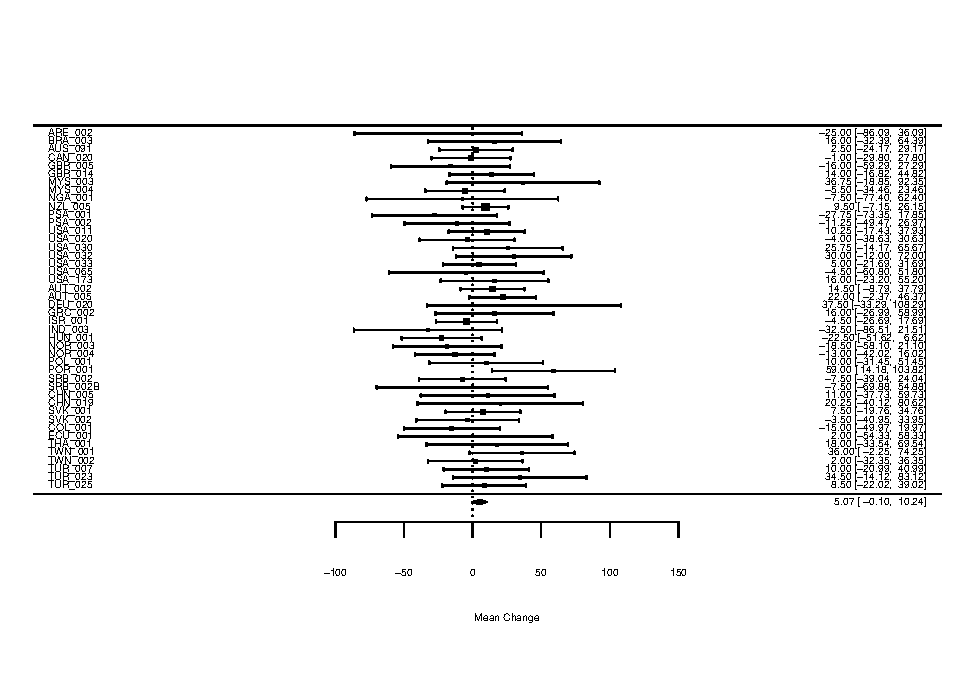
\includegraphics{Stage2_Report_0228_files/figure-latex/meta-all-1.pdf}
\caption{\label{fig:meta-all}Meta-analysis on match advantage of object orienation for all datasets}
\end{figure}

(Insert Figure \ref{fig:meta-all} about here)

\begin{figure}
\centering
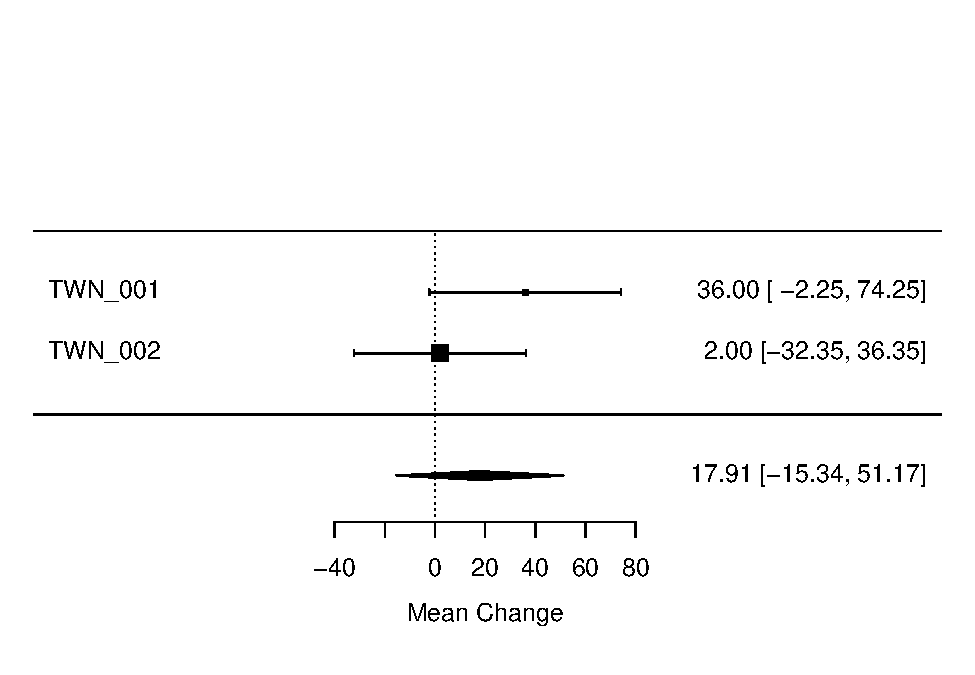
\includegraphics{Stage2_Report_0228_files/figure-latex/meta-tc-1.pdf}
\caption{\label{fig:meta-tc}Meta-analysis on match advantage of object orienation for Traditional Chinese datasets.}
\end{figure}

(Insert Figure \ref{fig:meta-tc} about here)

\begin{verbatim}
## [1] 916599.3
\end{verbatim}

\begin{verbatim}
## [1] 873794.4
\end{verbatim}

\begin{verbatim}
## [1] 871275.7
\end{verbatim}

\begin{verbatim}
## [1] 871086.4
\end{verbatim}

\begin{verbatim}
## [1] TRUE
\end{verbatim}

\begin{verbatim}
## [1] TRUE
\end{verbatim}

\begin{verbatim}
## [1] TRUE
\end{verbatim}

\begin{verbatim}
## [1] 871084.8
\end{verbatim}

\begin{verbatim}
## [1] TRUE
\end{verbatim}

\begin{verbatim}
## Linear mixed model fit by REML. t-tests use Satterthwaite's method [
## lmerModLmerTest]
## Formula: response_time ~ Match + (1 | Subject) + (1 | Target) + (1 | Language)
##    Data: SP_V_lme_data_excluded
## Control: lmerControl(optimizer = "bobyqa", optCtrl = list(maxfun = 1e+06))
## 
## REML criterion at convergence: 871072.8
## 
## Scaled residuals: 
##     Min      1Q  Median      3Q     Max 
## -5.2617 -0.6041 -0.0838  0.5342  7.0093 
## 
## Random effects:
##  Groups   Name        Variance Std.Dev.
##  Subject  (Intercept) 23652.5  153.79  
##  Target   (Intercept)   836.6   28.92  
##  Language (Intercept)  2011.4   44.85  
##  Residual             19778.3  140.64  
## Number of obs: 67567, groups:  Subject, 3317; Target, 48; Language, 18
## 
## Fixed effects:
##                   Estimate Std. Error        df t value Pr(>|t|)    
## (Intercept)        661.852     11.973    22.315  55.277   <2e-16 ***
## MatchMISMATCHING     1.376      1.087 64242.366   1.266    0.205    
## ---
## Signif. codes:  0 '***' 0.001 '**' 0.01 '*' 0.05 '.' 0.1 ' ' 1
## 
## Correlation of Fixed Effects:
##             (Intr)
## MMISMATCHIN -0.045
\end{verbatim}

\begin{verbatim}
## [1] 871088.3
\end{verbatim}

\begin{verbatim}
## [1] FALSE
\end{verbatim}

\begin{verbatim}
## Linear mixed model fit by REML. t-tests use Satterthwaite's method [
## lmerModLmerTest]
## Formula: response_time ~ Match + (1 | Subject) + (1 | Target) + (1 + Match |  
##     Language)
##    Data: SP_V_lme_data_excluded
## Control: lmerControl(optimizer = "bobyqa", optCtrl = list(maxfun = 1e+06))
## 
## REML criterion at convergence: 871072.3
## 
## Scaled residuals: 
##     Min      1Q  Median      3Q     Max 
## -5.2644 -0.6041 -0.0837  0.5342  7.0114 
## 
## Random effects:
##  Groups   Name             Variance  Std.Dev. Corr
##  Subject  (Intercept)      23652.739 153.7945     
##  Target   (Intercept)        836.579  28.9237     
##  Language (Intercept)       1974.114  44.4310     
##           MatchMISMATCHING     0.718   0.8473 1.00
##  Residual                  19778.158 140.6348     
## Number of obs: 67567, groups:  Subject, 3317; Target, 48; Language, 18
## 
## Fixed effects:
##                  Estimate Std. Error      df t value Pr(>|t|)    
## (Intercept)       661.655     11.881  22.278  55.691   <2e-16 ***
## MatchMISMATCHING    1.793      1.106 209.088   1.621    0.107    
## ---
## Signif. codes:  0 '***' 0.001 '**' 0.01 '*' 0.05 '.' 0.1 ' ' 1
## 
## Correlation of Fixed Effects:
##             (Intr)
## MMISMATCHIN 0.124 
## optimizer (bobyqa) convergence code: 0 (OK)
## boundary (singular) fit: see help('isSingular')
\end{verbatim}

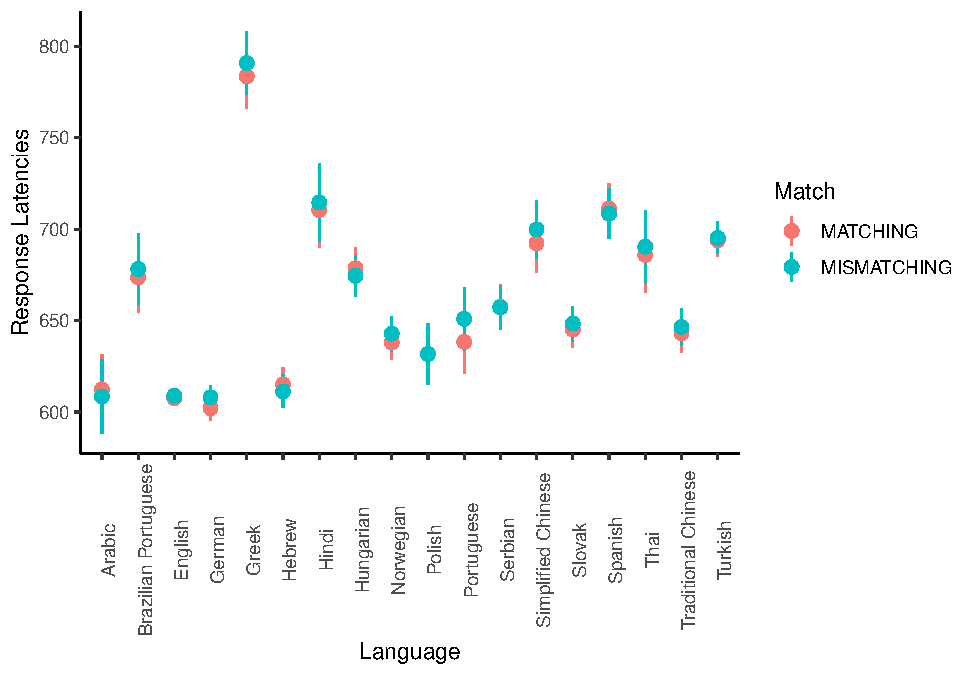
\includegraphics{Stage2_Report_0228_files/figure-latex/SP_lme_update-1.pdf} 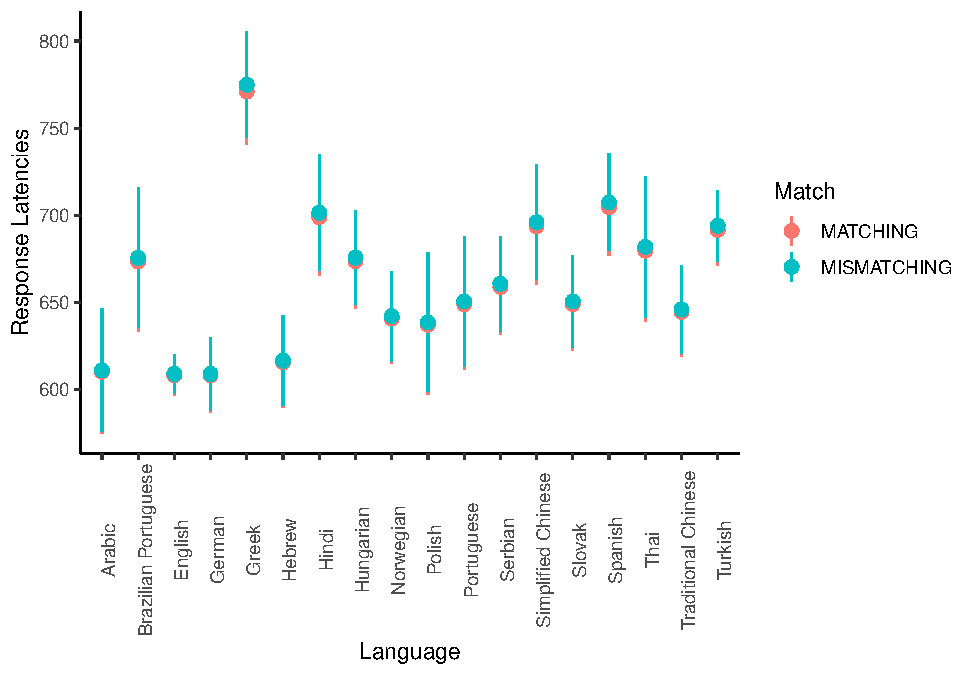
\includegraphics{Stage2_Report_0228_files/figure-latex/SP_lme_update-2.pdf}

\hypertarget{not-using-because-dont-need-the-split}{%
\subsection{not using because don't need the split}\label{not-using-because-dont-need-the-split}}

\textbf{Evaluating match advantages using linear mixed-effects models.} Considering the bias of small sample size, we excluded the languages with below 25 participants in each data source before conducting the mixed-effects models. Thus we excluded Portuguese in the on-site data and Norwegian in the web-based data. Because the sources of data collection included the labs and the web, we had to evaluate whether one mixed-effects model sufficiently fitted all the data. Otherwise, separate models would be needed for each data set. This analysis showed a significant difference between data sources: \emph{b} = 16.782, \emph{SE} = 15.232, t( 27.679 ) = 1.102, \emph{p} \textless{} .001. Thus, the on-site and the web-based data had to be analyzed separately.

The final models examined the interaction between language and match advantage in each data source, as reported below. All other models are reported in Appendix 4. It must be acknowledged that the languages with larger sample sizes (see Tables \ref{tab:summary-site} and \ref{tab:summary-osweb}) have more reliable results. Furthermore, most of the languages were underpowered, being far from the 1,200 participants suggested by an a priori power analysis.

In each data source, we compared the fit of the models with and without the random slope of matching condition. Both indicated that the models without the random slope had the best fit. The model from the on-site data revealed no significant effect of match advantage: \emph{b} = 2.898, \emph{SE} = 2.659, t( 38308.093 ) = 1.09, \emph{p} = 0.276. The model from the web-based data also failed to reveal a significant effect: \emph{b} = -8.496, \emph{SE} = 7.841, t( 25456.123 ) = -1.084, \emph{p} = 0.279. The latter model had a negative coefficient, unlike the on-site data. Although neither effect was significant, the difference in direction resounds with the match advantages and disadvantages found in experiments using the property of color (cf. Connell, 2007; Zwaan \& Pecher, 2012).

\begin{figure}
\centering
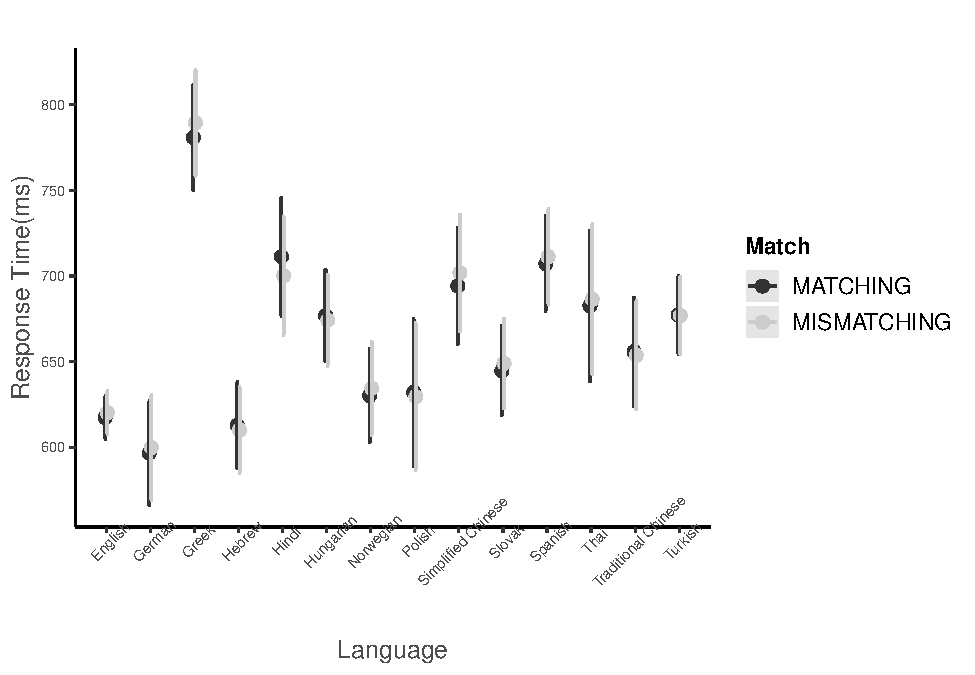
\includegraphics{Stage2_Report_0228_files/figure-latex/plot-SP-site-lme-1.pdf}
\caption{\label{fig:plot-SP-site-lme}Response times and standard error in the sentence-picture verification task by match condition in each language (on-site data only).}
\end{figure}

\begin{figure}
\centering
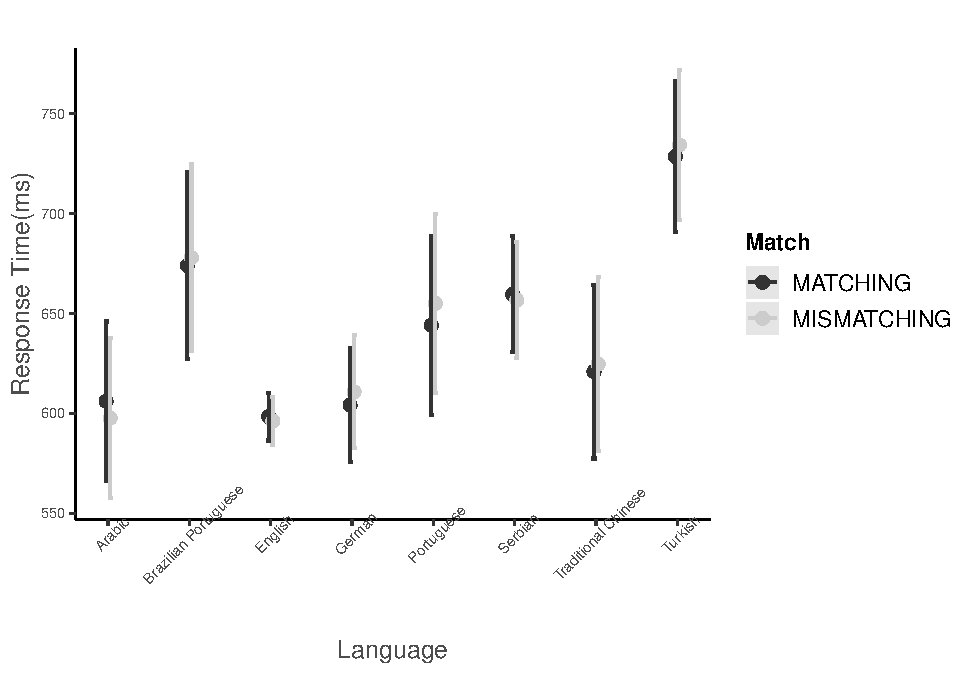
\includegraphics{Stage2_Report_0228_files/figure-latex/plot-SP-osweb-lme-1.pdf}
\caption{\label{fig:plot-SP-osweb-lme}Response times and standard error in the sentence-picture verification task by match condition in each language (web-based data only).}
\end{figure}

Figure \ref{fig:plot-SP-site-lme} illustrates the response times from the on-site data. Eight languages presented significant intercepts (see ``Models including languages'' section in Appendix 4).

(Insert Figure \ref{fig:plot-SP-site-lme} about here)

Figure \ref{fig:plot-SP-osweb-lme} illustrates the response times in the web-based data. Three languages presented significant effects (see ``Models included languages'' section in Appendix 4).

(Insert Figure \ref{fig:plot-SP-osweb-lme} about here)

\textbf{Anecdotal evidence on the match advantage.} In the on-site data, only Greek presented a match advantage, \emph{b} = 5.721, \emph{SE} = 7.204, t( 38316.593 ) = 0.794, \emph{p} = 0.427. It should be noted, however, that these results are not robust due to the underpowered sample sizes (see Discussion).

The mean response times in Greek (\emph{M} = 787.12, \emph{SD} = 272.75) and Serbian (\emph{M} = 657.38, \emph{SD} = 222.59) was longer than the average across languages (M = 640.54, SD = 213.56). This might not be coincidental, as according to Yap et al. (2014), longer response times have been associated with larger effects in psycholinguistics (Schilling et al., 1998; Seidenberg, 1985; Tainturier, 1992).

\textbf{Analysis of imagery scores.} Prior to data collection, we assumed the imagery scores of every language group would be nearly equal. The best-fitting model included random intercepts for participants, targets and laboratories but no slopes for orientation. The fixed effect of orientation match was significant, \emph{b} = 27.366, \emph{SE} = 2.275, t( 138198.589 ) = 12.032, \emph{p} \textless{} .001. The response times illustrated in Figure \ref{fig:plot-PP-lme} indicated that the imagery scores measured for each language were consistently positive supporting our hypothesis. The coefficients of all evaluated mixed-effects models are reported in Appendix 5.

(Insert Figure \ref{fig:plot-PP-lme} about here)

\begin{figure}
\centering
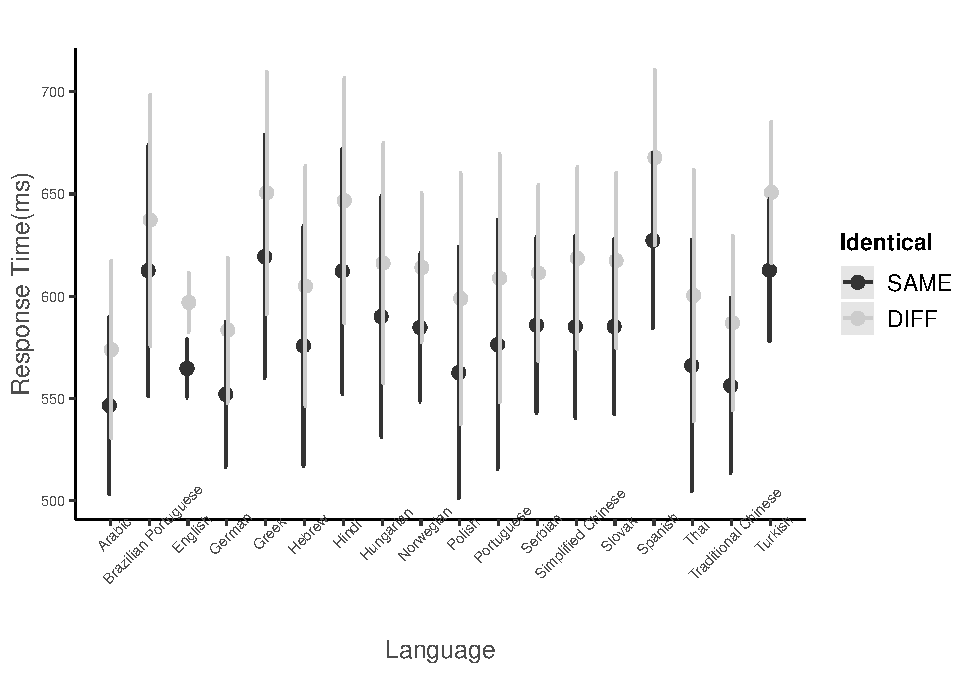
\includegraphics{Stage2_Report_0228_files/figure-latex/plot-PP-lme-1.pdf}
\caption{\label{fig:plot-PP-lme}Response times and standard error in the picture-picture verification task by match condition in each language (both on-site and web-based data).}
\end{figure}

The above analyses suggested that data sources did not influence the imagery scores but did influence the match advantage. Therefore, we evaluated the fit of the model with languages and imagery scores and the model with languages only. Both models included match advantage as the dependent variable. If imagery scores predict match advantage, the model with languages and imagery scores should fit the data better than the model with languages only. Because the random slopes for items in the analyses of the match advantage were zero (see Appendix 5), the data for building the regression models were the aggregated data by participants.

In the linear regression analysis, we decided the best fit model from the model with only predictor, language, and the model with two predictors, languages and imagery scores. Because the analysis of match advantage revealed the difference between data sources, we conducted the regression analysis by the data source respectively. In the analysis of the on-site data, the model with language and imagery scores had yet fit better than the model with language only, \emph{F} = 1.413, \emph{p} = 0.138. In contrast, in the analysis of the web-based data, the model with language and imagery scores had a better fit than the model with language only, \emph{F} (8,1266) = 0.623, \emph{p} =0.138. In the latter case, the effect of imagery scores was nonsignificant, \(b = -0.29\), 95\% CI \([-0.67, 0.09]\), \(t(1266) = -1.50\), \(p = .135\). Appendix 5 summarized the coefficients of the models included in these analyses.

\hypertarget{exploratory-analysis-language-specific-match-advantages}{%
\subsection{Exploratory analysis: language-specific match advantages}\label{exploratory-analysis-language-specific-match-advantages}}

Based on the policy to conduct the linguistic-specific mixed-effect models, we selected the English datasets (N = 1,346) and the Traditional Chinese datasets (N = 149). For both languages, we are interested in whether the data sources could inhibit the match advantage. Another topic of interest is if the match advantage changed with English dialects, namely American English and British English.

Using the data from 1,346 English speaking participants, we ran a mixed-effects model for the English data containing orientation match condition, English dialects (American vs.~British) and data sources (on-site vs.~web-based) as fixed effects. Following Brauer \& Curtin (2018), English dialects and data sources were numerically recoded. The best fitted model indicated that only data source (on-site vs.~web-based) was significant, \emph{b} = -8.622, \emph{SE} = 32.34, t( 16.613 ) = -0.267, \emph{p} \textless{} .001. Although the match advantage of orientation was nonsignificant, this exploratory analysis indicated the interaction of orientation match condition and English dialects: \emph{b} = 0.746, \emph{SE} = 4.735, t( 25929.071 ) = 0.158, \emph{p} = 0.875 (see the detailed report in Appendix 4).

We conducted another exploratory mixed-effect model on Traditional Chinese data because his was the only language to show a significant result in the preregistered meta-analysis. The best fit model had orientation match condition and data sources as the fixed effects. This model indicated that data source was significant, \emph{b} = 35.408, \emph{SE} = 25.786, t( 159.874 ) = 1.373, \emph{p} \textless{} .001. The match advantage of orientation was nearly significant: \emph{b} = 5.822, \emph{SE} = 8.336, t( 2852.347 ) = 0.698, \emph{p} = 0.4853, but the interaction of match advantage and data sources was nonsignificant: \emph{b} = -8.081, \emph{SE} = 10.619, t( 2852.841 ) = -0.761, \emph{p} = 0.447 (see the detailed report in Appendix 4). This result suggested that Traditional Chinese study could have a robust estimation in the circumstance multiple teams conducted the study in terms of one the same protocol. Combined with the previous results of Traditional Chinese (Chen et al., 2020), future research on this language could explore any potential linguistic aspects that might result in the match advantage of object orientation and other properties. Although this study is unable to provide further advice, the advantage for the future Traditional Chinese studies would be a precise sample size justification on the participants and stimulus items.

\newpage

\hypertarget{references}{%
\section{References}\label{references}}

\begingroup
\setlength{\parindent}{-0.5in}
\setlength{\leftskip}{0.5in}

\hypertarget{refs}{}
\begin{CSLReferences}{1}{0}
\leavevmode\vadjust pre{\hypertarget{ref-anwyl-irvineGorillaOurMidst2020}{}}%
Anwyl-Irvine, A. L., Massonnié, J., Flitton, A., Kirkham, N., \& Evershed, J. K. (2020). Gorilla in our midst: {An} online behavioral experiment builder. \emph{Behavior Research Methods}, \emph{52}(1), 388--407. \url{https://doi.org/10.3758/s13428-019-01237-x}

\leavevmode\vadjust pre{\hypertarget{ref-armstrongWhenUseBonferroni2014}{}}%
Armstrong, R. A. (2014). When to use the {Bonferroni} correction. \emph{Ophthalmic and Physiological Optics}, \emph{34}(5), 502--508. \url{https://doi.org/10.1111/opo.12131}

\leavevmode\vadjust pre{\hypertarget{ref-baayen_mixed-effects_2008}{}}%
Baayen, R. H., Davidson, D. J., \& Bates, D. M. (2008). Mixed-effects modeling with crossed random effects for subjects and items. \emph{Journal of Memory and Language}, \emph{59}(4), 390--412. \url{https://doi.org/10.1016/j.jml.2007.12.005}

\leavevmode\vadjust pre{\hypertarget{ref-batesFittingLinearMixedEffects2015}{}}%
Bates, D., Mächler, M., Bolker, B., \& Walker, S. (2015). Fitting {Linear Mixed}-{Effects Models Using} Lme4. \emph{Journal of Statistical Software}, \emph{67}(1). \url{https://doi.org/10.18637/jss.v067.i01}

\leavevmode\vadjust pre{\hypertarget{ref-brauerLinearMixedeffectsModels2018}{}}%
Brauer, M., \& Curtin, J. J. (2018). Linear mixed-effects models and the analysis of nonindependent data: {A} unified framework to analyze categorical and continuous independent variables that vary within-subjects and/or within-items. \emph{Psychological Methods}, \emph{23}(3), 389--411. \url{https://doi.org/10.1037/met0000159}

\leavevmode\vadjust pre{\hypertarget{ref-bridgesTimingMegastudyComparing2020a}{}}%
Bridges, D., Pitiot, A., MacAskill, M. R., \& Peirce, J. W. (2020). The timing mega-study: Comparing a range of experiment generators, both lab-based and online. \emph{PeerJ}, \emph{8}, e9414. \url{https://doi.org/10.7717/peerj.9414}

\leavevmode\vadjust pre{\hypertarget{ref-chenDoesObjectSize2020}{}}%
Chen, S.-C., de Koning, B. B., \& Zwaan, R. A. (2020). Does object size matter with regard to the mental simulation of object orientation? \emph{Experimental Psychology}, \emph{67}(1), 56--72. \url{https://doi.org/10.1027/1618-3169/a000468}

\leavevmode\vadjust pre{\hypertarget{ref-connellRepresentingObjectColour2007}{}}%
Connell, L. (2007). Representing object colour in language comprehension. \emph{Cognition}, \emph{102}, 476--485. \url{https://doi.org/10.1016/j.cognition.2006.02.009}

\leavevmode\vadjust pre{\hypertarget{ref-deleeuwPsychophysicsWebBrowser2016}{}}%
de Leeuw, J. R., \& Motz, B. A. (2016). Psychophysics in a {Web} browser? {Comparing} response times collected with {JavaScript} and {Psychophysics Toolbox} in a visual search task. \emph{Behavior Research Methods}, \emph{48}(1), 1--12. \url{https://doi.org/10.3758/s13428-015-0567-2}

\leavevmode\vadjust pre{\hypertarget{ref-kosterMentalSimulationObject2018}{}}%
Koster, D., Cadierno, T., \& Chiarandini, M. (2018). Mental simulation of object orientation and size: {A} conceptual replication with second language learners. \emph{Journal of the European Second Language Association}, \emph{2}(1). \url{https://doi.org/10.22599/jesla.39}

\leavevmode\vadjust pre{\hypertarget{ref-kuznetsovaLmerTestPackageTests2017}{}}%
Kuznetsova, A., Brockhoff, P. B., \& Christensen, R. H. B. (2017). {\textbf{lmerTest}} {Package}: {Tests} in {Linear Mixed Effects Models}. \emph{Journal of Statistical Software}, \emph{82}(13). \url{https://doi.org/10.18637/jss.v082.i13}

\leavevmode\vadjust pre{\hypertarget{ref-langeJustAnotherTool2015}{}}%
Lange, K., Kühn, S., \& Filevich, E. (2015). "{Just Another Tool} for {Online Studies}'' ({JATOS}): {An} easy solution for setup and management of web servers supporting online studies. \emph{PLOS ONE}, \emph{10}(6), e0130834. \url{https://doi.org/10.1371/journal.pone.0130834}

\leavevmode\vadjust pre{\hypertarget{ref-lukeEvaluatingSignificanceLinear2017}{}}%
Luke, S. G. (2017). Evaluating significance in linear mixed-effects models in {R}. \emph{Behavior Research Methods}, \emph{49}(4), 1494--1502. \url{https://doi.org/10.3758/s13428-016-0809-y}

\leavevmode\vadjust pre{\hypertarget{ref-mathotOpenSesameOpensourceGraphical2012}{}}%
Mathôt, S., Schreij, D., \& Theeuwes, J. (2012). {OpenSesame}: {An} open-source, graphical experiment builder for the social sciences. \emph{Behavior Research Methods}, \emph{44}(2), 314--324. \url{https://doi.org/10.3758/s13428-011-0168-7}

\leavevmode\vadjust pre{\hypertarget{ref-moshontzPsychologicalScienceAccelerator2018}{}}%
Moshontz, H., Campbell, L., Ebersole, C. R., IJzerman, H., Urry, H. L., Forscher, P. S., Grahe, J. E., McCarthy, R. J., Musser, E. D., Antfolk, J., Castille, C. M., Evans, T. R., Fiedler, S., Flake, J. K., Forero, D. A., Janssen, S. M. J., Keene, J. R., Protzko, J., Aczel, B., \ldots{} Chartier, C. R. (2018). The {Psychological Science Accelerator}: {Advancing} psychology through a distributed collaborative network. \emph{Advances in Methods and Practices in Psychological Science}, \emph{1}(4), 501--515. \url{https://doi.org/10.1177/2515245918797607}

\leavevmode\vadjust pre{\hypertarget{ref-schillingComparingNamingLexical1998}{}}%
Schilling, H. E. H., Rayner, K., \& Chumbley, J. I. (1998). Comparing naming, lexical decision, and eye fixation times: {Word} frequency effects and individual differences. \emph{Memory \& Cognition}, \emph{26}(6), 1270--1281. \url{https://doi.org/10.3758/BF03201199}

\leavevmode\vadjust pre{\hypertarget{ref-schonbrodtSequentialHypothesisTesting2017}{}}%
Schönbrodt, F. D., Wagenmakers, E.-J., Zehetleitner, M., \& Perugini, M. (2017). Sequential hypothesis testing with {Bayes} factors: {Efficiently} testing mean differences. \emph{Psychological Methods}, \emph{22}(2), 322--339. \url{https://doi.org/10.1037/met0000061}

\leavevmode\vadjust pre{\hypertarget{ref-seidenbergTimeCoursePhonological1985}{}}%
Seidenberg, M. (1985). The time course of phonological code activation in two writing systems. \emph{Cognition}, \emph{19}(1), 1--30. \url{https://doi.org/10.1016/0010-0277(85)90029-0}

\leavevmode\vadjust pre{\hypertarget{ref-stanfield_effect_2001}{}}%
Stanfield, R. A., \& Zwaan, R. A. (2001). The effect of implied orientation derived from verbal context on picture recognition. \emph{Psychological Science}, \emph{12}(2), 153--156. \url{https://doi.org/10.1111/1467-9280.00326}

\leavevmode\vadjust pre{\hypertarget{ref-tainturierEducationalLevelWord1992}{}}%
Tainturier, M. (1992). Educational level and the word frequency effect: {A} lexical decision investigation*1. \emph{Brain and Language}, \emph{43}(3), 460--474. \url{https://doi.org/10.1016/0093-934X(92)90112-R}

\leavevmode\vadjust pre{\hypertarget{ref-viechtbauerConductingMetaAnalysesMetafor2010}{}}%
Viechtbauer, W. (2010). Conducting {Meta}-{Analyses} in {R} with the metafor {Package}. \emph{Journal of Statistical Software}, \emph{36}(1), 1--48. \url{https://doi.org/10.18637/jss.v036.i03}

\leavevmode\vadjust pre{\hypertarget{ref-yapRespondingNonwordsLexical2014}{}}%
Yap, M. J., Sibley, D. E., Balota, D. A., Ratcliff, R., \& Rueckl, J. (2014). Responding to nonwords in the lexical decision task: Insights from the {English Lexicon Project}. \emph{Journal of Experimental Psychology: Learning, Memory, and Cognition}, No Pagination Specified. \url{https://doi.org/10.1037/xlm0000064}

\leavevmode\vadjust pre{\hypertarget{ref-zwaanRevisitingMentalSimulation2012}{}}%
Zwaan, R. A., \& Pecher, D. (2012). Revisiting mental simulation in language comprehension: Six replication attempts. \emph{PLoS ONE}, \emph{7}, e51382. \url{https://doi.org/10.1371/journal.pone.0051382}

\end{CSLReferences}

\endgroup


\end{document}
